\documentclass{article}
\usepackage[top=8mm, bottom=8mm, inner=8mm, outer=8mm, 
headheight=0mm, headsep=0mm, footskip=0mm, 
%papersize={148mm, 210mm},
papersize={297mm, 210mm},
includeheadfoot
]{geometry}
\usepackage{tikz}
\usepackage{lipsum}
\usepackage{fontspec}
\pagestyle{empty}

\setmainfont{Libertinus Sans}

\newcommand{\CDtitle}[1]{
{\setmainfont{Raleway SemiBold}\LARGE #1}\par
}

\setlength{\parindent}{0cm}

\newcommand{\CDsubtitle}[1]{
\par\medskip
{\setmainfont{Raleway SemiBold}\large #1}
\par
}

\begin{document}
\begin{minipage}[t][192mm]{132mm}
\CDtitle{How to drive a punt}
\CDsubtitle{10 Get in the boat}
\vspace{-4mm}
\begin{center}
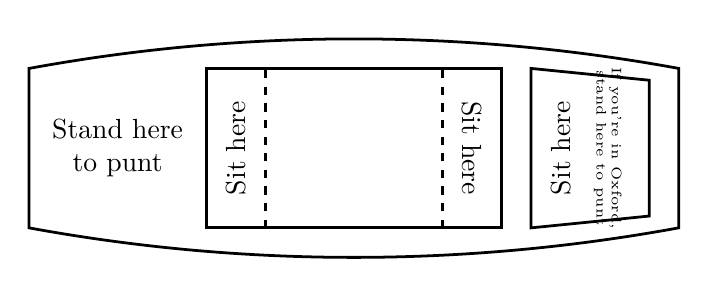
\begin{tikzpicture}[x=0.75cm,y=0.75cm]
%\draw[line width=1pt] (5,0) -- (5,2);
%\draw[line width=1pt] (0,0) -- (0,2);
\draw[line width=1pt] (0,0) arc (-100.39:-79.61:30.5) -- (11,0) -- (11,2.7) arc (79.61:100.39:30.5) -- (0,2.7) -- cycle;
\draw[line width=1pt] (3,0) rectangle (8,2.7);
\draw[line width=1pt] (8.5,0) -- (10.5,0.2) -- (10.5,2.5) -- (8.5,2.7) -- cycle;
\draw[line width=1pt,dashed] (7,0) -- (7,2.7);
\draw[line width=1pt,dashed] (4,0) -- (4,2.7);
\node[rotate=90] at (3.5,1.35) {Sit here};
\node[rotate=-90] at (7.5,1.35) {Sit here};
\node[rotate=90] at (9,1.35) {Sit here};
\node[align=center] at (1.5,1.35) {Stand here\\to punt};
\node[align=center,rotate=-90] at (9.8,1.35) {\tiny If you're in Oxford,\\[-2.3mm]\tiny stand here to punt};
%\draw[line width=2pt] (0,0) -- plot[domain=4.44:4.98,variable=\t]({2.5+1*9.34*cos(\t r)},{9 + 9.34*sin(\t r)});
\end{tikzpicture}
\end{center}

\vfill

\CDsubtitle{20 Drop the pole vertically into the water beside the boat}
\vspace{-3mm}
\begin{center}
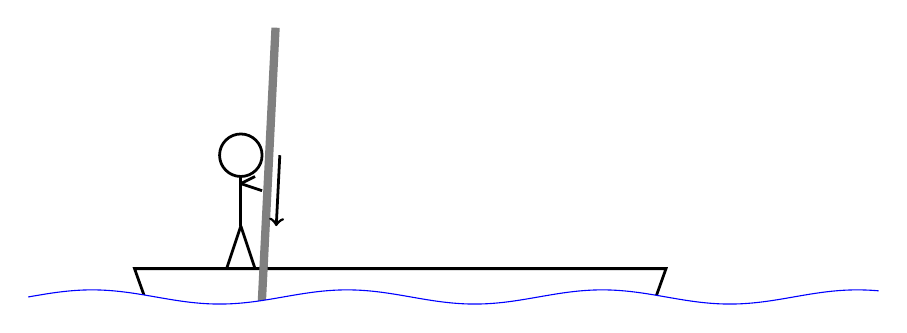
\begin{tikzpicture}[x=0.9cm,y=0.9cm]
\begin{scope}
\clip (0,3.8) -- plot[domain=0:12,samples=500,variable=\x] ({\x},{0.1*sin(\x*100)}) -- (12,3.8) -- cycle;
\draw[line width=1pt] (2,-1) -- (1.5,0.4) -- (9,0.4) -- (8.5,-1);
\draw[line width=1pt] (3,2) circle (0.3);
\draw[line width=1pt] (3,1.7) -- (3,1);
\draw[line width=1pt] (2.8,0.4) -- (3,1);
\draw[line width=1pt] (3.2,0.4) -- (3,1);
\draw[line width=1pt] (3,1.6) -- (3.2,1.7);
\draw[line width=3pt, gray] (3.49,3.8) -- (3.25,-1);
\draw[line width=1pt] (3.3,1.5) -- (3,1.6);
\end{scope}
\draw[blue] plot[domain=0:12,samples=500,variable=\x] ({\x},{0.1*sin(\x*100)});
\draw[line width=1pt,->] (3.55,2) -- (3.5,1);
\end{tikzpicture}
\end{center}

\vfill

\CDsubtitle{30 Catch pole and push forward off the bottom of the river}
\vspace{-6mm}
\begin{center}
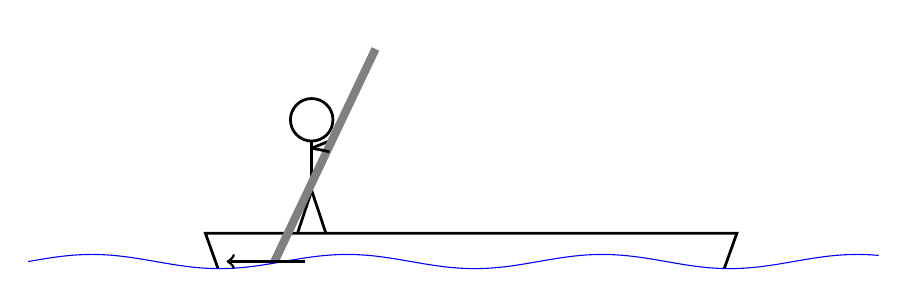
\begin{tikzpicture}[x=0.9cm,y=0.9cm]
\begin{scope}
\clip (0,3.3) -- plot[domain=0:12,samples=500,variable=\x] ({\x},{0.1*sin(\x*100)}) -- (12,3.3) -- cycle;
\begin{scope}[shift={(1,0)}]
\draw[line width=1pt] (2,-1) -- (1.5,0.4) -- (9,0.4) -- (8.5,-1);
\draw[line width=1pt] (3,2) circle (0.3);
\draw[line width=1pt] (3,1.7) -- (3,1);
\draw[line width=1pt] (2.8,0.4) -- (3,1);
\draw[line width=1pt] (3.2,0.4) -- (3,1);
\draw[line width=1pt] (3,1.6) -- (3.25,1.7);
\draw[line width=3pt, gray] (3.9,3) -- (2,-1);
\draw[line width=1pt] (3.25,1.55) -- (3,1.6);
\end{scope}
\end{scope}
\draw[blue] plot[domain=0:12,samples=500,variable=\x] ({\x},{0.1*sin(\x*100)});
\draw[line width=1pt,->] (3.9,0) -- (2.8,0);
\end{tikzpicture}
\end{center}

\vfill

\CDsubtitle{40 Let the boat glide along the river, using the pole to steer}
\begin{center}
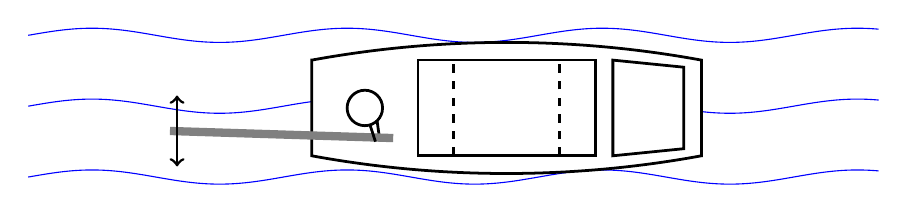
\begin{tikzpicture}[x=0.9cm,y=0.9cm]
\draw[blue] plot[domain=0:12,samples=500,variable=\x] ({\x},{0.1*sin(\x*100)});
\draw[blue] plot[domain=0:12,samples=500,variable=\x] ({\x},{1+0.1*sin(\x*100)});
\draw[blue] plot[domain=0:12,samples=500,variable=\x] ({\x},{2+0.1*sin(\x*100)});
\begin{scope}[shift={(4,0.3)},scale=0.5]
\draw[line width=1pt,fill=white] (0,0) arc (-100.39:-79.61:30.5) -- (11,0) -- (11,2.7) arc (79.61:100.39:30.5) -- (0,2.7) -- cycle;
\draw[line width=1pt] (3,0) rectangle (8,2.7);
\draw[line width=1pt] (8.5,0) -- (10.5,0.2) -- (10.5,2.5) -- (8.5,2.7) -- cycle;
\draw[line width=1pt,dashed] (7,0) -- (7,2.7);
\draw[line width=1pt,dashed] (4,0) -- (4,2.7);

\draw[line width=1pt] (1.8,1.31) -- (1.9,0.6);
\draw[line width=3pt, gray] (2.3,0.5) -- (-4,0.7);
\draw[line width=1pt] (1.5,1.31) -- (1.8,0.4);
\draw[line width=1pt,fill=white] (1.5,1.35) circle (0.5);
\draw[line width=1pt,<->] (-3.8,-0.3) -- (-3.8,1.7);
\end{scope}
\end{tikzpicture}
\end{center}

\vfill

\CDsubtitle{50 Lift pole upwards out of water}

\vfill

\CDsubtitle{60 GOTO 20}

\vfill

Note: You don't need to use the paddle unless you lose the pole (if you do lose the pole, you can use the paddle to go back and get it).

\end{minipage}%
\hfill%
\begin{minipage}[t][192mm]{132mm}
Hello there!

\vfill

General Kenobi!
\end{minipage}

\newpage

\lipsum
\end{document}
